\documentclass[11pt]{article}

\usepackage[a4paper,margin=1in]{geometry}
\usepackage{amsmath, amssymb}
\usepackage{microtype}
\usepackage{newpxtext, newpxmath}
\usepackage{xcolor}
\usepackage[most]{tcolorbox}
\usepackage{enumitem}
\usepackage{titlesec}
\usepackage{tikz}
\usetikzlibrary{positioning, arrows.meta}

\definecolor{inkblue}{HTML}{1F3A5F}
\definecolor{boxbg}{HTML}{F2F5F9}
\definecolor{boxrule}{HTML}{8AA4C4}

\titleformat{\section}{\large\bfseries\color{inkblue}}{}{0em}{}
\titlespacing{\section}{0pt}{1.4em}{0.5em}

\newtcolorbox{insight}{
  colback=boxbg, colframe=boxrule, boxrule=0.6pt,
  arc=2pt, left=10pt, right=10pt, top=8pt, bottom=8pt,
  breakable, enhanced,
  title={\textbf{Insight}}, coltitle=inkblue, fonttitle=\bfseries\small,
  attach title to upper=\hspace{0.6em}
}

\newtcolorbox{summary}{colback=yellow!18, colframe=yellow!55!black, arc=2pt, boxrule=0.5pt,
  breakable, left=10pt, right=10pt, top=8pt, bottom=8pt}

\setlength{\parskip}{0.55em}
\setlength{\parindent}{0pt}

\title{\color{inkblue}\bfseries Four Shadows}
\author{One convex function, seen four ways}
\date{}

\begin{document}
\maketitle
\thispagestyle{empty}

One could sum up this whole document in a sentence:
\begin{summary}
The four companion notes are not four subjects. They are one object --- the convex function
$A(z) = \log\sum_k e^{z_k}$ --- lit from four sides. Its value, its gradient, its dual, its
Hessian, and its Bregman divergence are, respectively, the normaliser, the probabilities, the
entropy, the metric, and the loss. Each note is a shadow; this one is the solid.
\end{summary}
\emph{Next-Token Prediction is Geometry}, \emph{Training is a Monte Carlo Estimate}, \emph{The
Radon--Nikodym Theorem}, and \emph{The Metric the Others Were Using} were written as four
separate investigations. They kept colliding with the same matrix, the same normaliser, the
same $\log\sum\exp$. This note explains why they had to: there was only ever one function
underneath, and they were walking around it.

\section{The solid, and its shadows}

\begin{center}
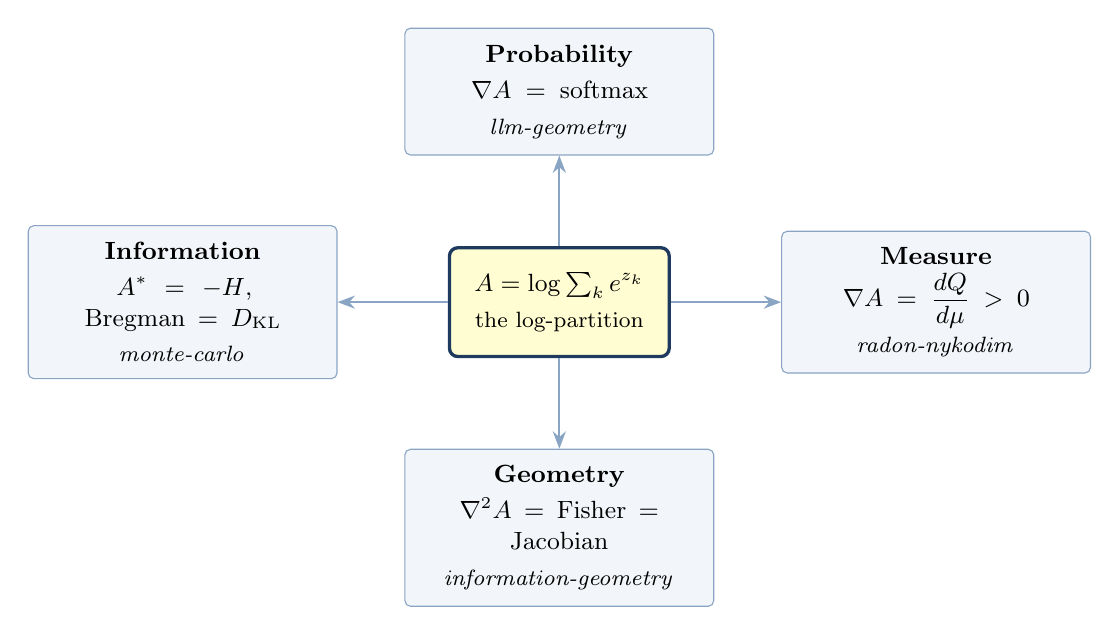
\begin{tikzpicture}[
  font=\small,
  core/.style={draw=inkblue, fill=yellow!18, rounded corners=3pt, very thick, align=center,
    inner sep=9pt},
  shadow/.style={draw=boxrule, fill=boxbg, rounded corners=2pt, align=center, inner sep=6pt,
    text width=3.5cm},
  link/.style={-{Stealth[length=2.2mm]}, draw=boxrule, thick}
]
  \node[core] (A) {$A=\log\sum_k e^{z_k}$\\[2pt]\footnotesize the log-partition};
  \node[shadow, above=1.15cm of A] (prob)
    {\textbf{Probability}\\[2pt]$\nabla A=\operatorname{softmax}$\\[2pt]\footnotesize\emph{llm-geometry}};
  \node[shadow, below=1.15cm of A] (geo)
    {\textbf{Geometry}\\[2pt]$\nabla^2 A=\text{Fisher}=\text{Jacobian}$\\[2pt]\footnotesize\emph{information-geometry}};
  \node[shadow, left=1.4cm of A] (info)
    {\textbf{Information}\\[2pt]$A^{*}=-H$,\ \ $\mathrm{Bregman}=D_{\mathrm{KL}}$\\[2pt]\footnotesize\emph{monte-carlo}};
  \node[shadow, right=1.4cm of A] (meas)
    {\textbf{Measure}\\[2pt]$\nabla A=\dfrac{dQ}{d\mu}>0$\\[2pt]\footnotesize\emph{radon-nykodim}};
  \draw[link] (A) -- (prob);
  \draw[link] (A) -- (geo);
  \draw[link] (A) -- (info);
  \draw[link] (A) -- (meas);
\end{tikzpicture}
\end{center}

Read the figure as one object casting four shadows. The same $A$ projects onto a probability,
a code length, a density, and a metric depending only on which wall you let the light fall on.

\section{The ladder of derivatives}

Take $A(z) = \log\sum_k e^{z_k}$ and simply read off what each standard operation on it
produces. Every row is a result from one of the four notes; the point is that they are all
rows of \emph{one} table.

\begin{itemize}[leftmargin=1.5em, itemsep=4pt]
  \item \textbf{The function itself}, $A(z)$ --- the normaliser, the $\log$ of the partition
  function $\sum_k e^{z_k}$ that turns raw logits into something that sums to one.
  \item \textbf{Its gradient}, $\nabla A(z) = \operatorname{softmax}(z) = p$ --- the
  probability distribution. The ``one-equation bridge'' of \emph{llm-geometry}, and the density
  $dQ/d\mu$ of \emph{radon-nykodim}, are both this single gradient. It is strictly positive
  because $A$ is finite and smooth, which is exactly why absolute continuity never fails.
  \item \textbf{Its Legendre dual}, $A^{*}(p) = \sup_z\bigl(\langle z,p\rangle - A(z)\bigr) =
  \sum_w p_w \log p_w = -H(p)$ --- the negative entropy. The irreducible floor of
  \emph{monte-carlo} is the conjugate of the normaliser.
  \item \textbf{Its Bregman divergence}, the gap between $A^{*}$ and its own tangent plane,
  $B_{A^{*}}(p \,\|\, q) = D_{\mathrm{KL}}(p \,\|\, q)$ --- the loss. Cross-entropy minus
  entropy, the extra bits of the wrong code, is the Bregman divergence of the dual potential.
  \item \textbf{Its Hessian}, $\nabla^2 A(z) = \operatorname{diag}(p) - p p^{\top}$ --- the
  Fisher information metric. This is simultaneously the softmax Jacobian $\partial p/\partial
  z$ that drove the spring-law gradient and the second-order curvature of $D_{\mathrm{KL}}$.
  One matrix; three notes had already written it down.
  \item \textbf{Its flatness in dual coordinates} --- $A$ is flat in the natural coordinates
  $z$ (the logits) and its dual $A^{*}$ is flat in the expectation coordinates $p$ (the
  probabilities). Those two flatnesses are the exponential and mixture connections, the
  dually-flat structure of \emph{information-geometry}.
\end{itemize}

\begin{summary}
\[
  A \;\rightsquigarrow\; \text{normaliser},\quad
  \nabla A \;\rightsquigarrow\; \text{softmax / density},\quad
  A^{*} \;\rightsquigarrow\; -\,\text{entropy},
\]
\[
  B_{A^{*}} \;\rightsquigarrow\; \text{KL loss},\quad
  \nabla^2 A \;\rightsquigarrow\; \text{Fisher metric} = \text{Jacobian} = \nabla^2 D_{\mathrm{KL}},\quad
  \text{dual-flat} \;\rightsquigarrow\; e\text{- and }m\text{-connections}.
\]
\end{summary}

\section{Why it is \emph{this} function}

The collapse is not luck. $A = \log\sum\exp$ is the \emph{cumulant generating function} of the
categorical exponential family --- the family softmax belongs to, with the logits as natural
parameters. For any such family three facts are automatic, and they are the three facts the
notes kept rediscovering:
\begin{itemize}[leftmargin=1.5em]
  \item the gradient of the cumulant generating function is the \textbf{mean} of the
  sufficient statistic --- here, $\nabla A = p$, the distribution itself;
  \item its Hessian is the \textbf{covariance} of that statistic --- here, $\operatorname{diag}(p)
  - pp^{\top}$, which is the definition of the Fisher metric;
  \item it is \textbf{convex}, so it has a Legendre dual, and convex duality pairs the two
  coordinate systems (logits and probabilities), the two potentials ($A$ and $-H$), and the two
  flat connections.
\end{itemize}
So the moment a model ends in a softmax, it has committed to an exponential family, and an
exponential family \emph{is} a convex potential wearing probability's clothes. Everything the
four notes measure --- likelihood, surprise, bits, density, distance, curvature --- is some
derivative or dual or divergence of that one potential. There was no way for them \emph{not} to
meet.

\begin{insight}
This is why the softmax Jacobian turning out to be the Fisher metric felt like a coincidence
and is not one: $\nabla A$ is softmax and $\nabla^2 A$ is both its Jacobian and the covariance
(the Fisher metric), because differentiating the gradient of $A$ is, tautologically,
differentiating softmax. The ``four shadows'' are four derivatives of one function, and
derivatives of a smooth function are not independent of each other --- they are the same
function's local data at successive orders.
\end{insight}

\section{Four lenses, one object}

The four notes are the object seen through four disciplines' lenses, and each discipline
names the shadow in its own vocabulary:
\begin{itemize}[leftmargin=1.5em]
  \item \textbf{Probability} (\emph{llm-geometry}) sees $\nabla A$ and calls it the next-token
  distribution; alignment in a vector space becomes likelihood.
  \item \textbf{Information theory} (\emph{monte-carlo}) sees $A^{*}$ and its Bregman gap and
  calls them entropy and the extra bits of a wrong code.
  \item \textbf{Measure theory} (\emph{radon-nykodim}) sees $\nabla A$ as a density $dQ/d\mu$,
  asks when it exists, and finds softmax's positivity answers the question before it is asked.
  \item \textbf{Differential geometry} (\emph{information-geometry}) sees $\nabla^2 A$ as a
  Riemannian metric and its dual flatness as a pair of connections.
\end{itemize}
The shadows look nothing alike --- a probability, a bit count, a density, a tensor --- which is
precisely why four separate notes could be written without their author noticing he was circling
one function. The casting object is identical in all four; only the wall changes.

\begin{insight}
Honest coda, carried over from the last note: this is \emph{recognised} structure, not
discovered. That a cumulant generating function's gradient is the mean, its Hessian the
covariance / Fisher metric, and its Bregman divergence the KL --- and that exponential families
are therefore dually flat --- is the organising spine of convex duality and information
geometry (Wainwright--Jordan; Amari). Nothing here is a new theorem. What these five documents
add is the map: the single sentence that the softmax, the loss, the density, and the metric are
one convex function's shadows, said plainly enough that the next reader does not have to circle
the object four times to see it.
\end{insight}

\section{Older than the thing it explains}

The dates are worth stating, because they invert the natural way of telling this. Rao made
Fisher information a Riemannian metric in 1945; Amari's dual connections were complete by the
1980s; the transformer is 2017. The structure predates the language model by forty to eighty
years, and so the honest ordering is the reverse of the usual one. It is tempting to say ``the
language model has a Fisher metric.'' In fact the Fisher metric is the general object and the
model is a late, narrow instance that fell into it. The softmax did not acquire this geometry
by being part of a network; it inherited it by being a categorical exponential family --- the
thing Fisher, Rao and Amari studied in full generality with no network anywhere in sight.

Why was the house already built? Not luck. This structure is the theory of \emph{any}
normalised parametric probability model fitted by maximum likelihood, and the three choices that
make a language model trainable at all are exactly the axioms that place it in that theory:
\begin{itemize}[leftmargin=1.5em]
  \item a \textbf{softmax} output makes it an exponential family (logits as natural parameters);
  \item a \textbf{cross-entropy} loss makes its objective the KL / Bregman divergence of that family;
  \item \textbf{maximum likelihood} by gradient descent moves it in the dual coordinate system
  the geometry describes.
\end{itemize}
No one chose these because they knew information geometry. They were chosen because they are the
differentiable, normalised, convex-per-example options that let gradient descent work --- and
``differentiable, normalised, maximum-likelihood'' \emph{is} the definition of the exponential
family. Anything trainable this way arrives at the same address. The 1945 mathematics was
waiting because it was never about neural networks; it was about the shape of ``fit a
probability model by likelihood,'' and that shape is older and far more general than the thing
now filling it.

That also draws the one line worth drawing --- between what the old mathematics settles and what
it leaves open. On the output-and-objective side, everything is settled and classical: why
cross-entropy is the right loss, the local geometry of that loss, the natural gradient, the fact
that the softmax Jacobian is the metric. On the far side of the \emph{network} Jacobian, nothing
is: why stochastic gradient descent on a transformer finds a good point, what the hidden layers
represent, why scale produces the behaviour it does. The parameter-space Fisher is this note's
metric pulled back through the network, $F_\theta = J_{\mathrm{net}}^{\top} g\, J_{\mathrm{net}}$,
and $J_{\mathrm{net}}$ is the new, un-theorised object. The classical theory owns the last layer
and the loss with total authority and says essentially nothing about the network that computes
the logits. The mystery did not vanish; it moved off the output layer, where the old masters had
mapped everything, onto the representation, where no one has.

\begin{summary}
C.\,R.~Rao, who turned Fisher information into a Riemannian metric in 1945, died in 2023 at the
age of 102 --- he lived to see the models arrive into the geometry he had given them
seventy-eight years earlier. Shun-ichi Amari, who built the dual-connection structure, is in his
late eighties. The tools predate the technology by a lifetime, and at least one of the
toolmakers was still here to watch it walk into the room he had furnished.
\end{summary}

\end{document}
